% 从现在起,你将扮演一位科研工作者,有着丰富的论文写作经验。现在有学生向你请教论文写作的问题。可能会给你一段话,你将这段话用英文润色;也可能是直接请教你一些表达或科技论文的框架。你的最终目的是,指导该学生写出一篇优秀的、可发表的科技论文。

\documentclass{article}
\usepackage{graphicx} % Required for inserting images
\usepackage{enumerate}
\usepackage{amsmath}
\usepackage{bm}
\usepackage[ruled,linesnumbered]{algorithm2e}

\def\T{\mathrm{T}}


\title{Greedy-based RBS maximum allowable current calculation method}
\author{3057761608 }
\date{March 2023}

\begin{document}

\maketitle

\section{Introduction}

% Battery energy storage systems(BESS) 被用在新能源汽车、风力发电站等场景中,为设备提供高品位电能的保存和释放。
Battery Energy Storage Systems (BESSs) are widely used to store and supply high-quality electrical energy in various applications, including electric vehicles and wind power turbines. 
Typically, a BESS consists of a large number of battery cells that are interconnected by series-parallel circuitry to provide the required charge storage capacity and output voltage. 
However, as the number of cells increases, the reliability of the system becomes a major concern. 
The capacity and safety of the BESS are mainly determined by the least healthy battery cells, a phenomenon known as the cask effect. 
Furthermore, the degradation of cells in poor condition is accelerated by multiple charge/discharge cycles, which can lead to early failure of the unhealthy cells. 
These limitations and issues are particularly problematic for traditional BESSs with fixed circuitry, which hinder their practical applications. 


% 【RBS的先进性、现状】
% Reconfigurable battery system(RBS) 解决固定电路电池组的 cask effect:系统的容量和寿命取决于状态最差的某些电池。
% 此外,不一致性也在系统运行中加剧恶化。
% 通过动态改变电路,调控或隔离不良电池,有助于提升系统整体可靠性。
% 但是,重构也增加了设计、分析和控制的难度。
% 当前,系统有成百上千的电池,平均每个电池由3~5个开关控制,形成了庞大的状态空间。
Reconfigurable Battery System (RBS), which can dynamically  switch between different circuit configurations as required, is expected to solve the above problem. 
Unlike fixed BESSs, reconfigurable circuits use additional switches to change the series/parallel relationship between batteries.
Figure 1 illustrates one of the classic architecture proposed by Visairo et al.\cite{visairoReconfigurableBatteryPack2008}.
When the longitudinal switches are cloesd and the diagonal switches are open, the batteries are connected in parallel; conversely, they are connected in series.
And any battery in the Figure can be disconnected to isolated the unhealthy one or to provide redundancy.
Based on the reconfiguration, RBSs are available to isolated the unhealthy batteries timely and balance the degradation differents between individual cells as required.
However, the reconfiguration also increases the complexity of system design and control.
Each battery in RBSs is controlled by an average of 3 to 5 switches according to reported architectures(ref:13-20).
When the system has hundreds or thousands of cells, there is a huge state space waits to solve.

\begin{figure}
    \centering
    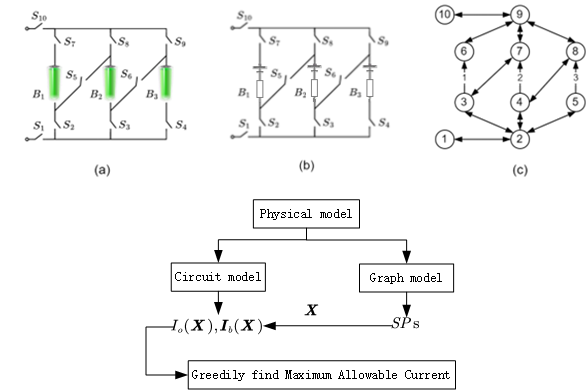
\includegraphics[width=\textwidth]{../attachments/fig1.png}
    \caption{The physical model (a), circuit model (b) and figure model(c) of the classic architecture reported by ref. (d) The overall framework of our method.}
    \label{fig:1}
\end{figure}


% 【快速评估系统最大电流的作用和意义、文献现状】
% (一些典型结构、控制策略、评估)
% 快速评估系统最大允许电流在设计、分析和控制中起到重要作用。
% 对设计,系统的最大输出电流
% 对控制,应对故障,静态结构破坏
% 但是没有严谨研究最大电流。(直接说没有)
% del: 一些研究使用了过度的简化,不准;(具体文献?):led
% del: 只针对小数量的电池和特定的结构,不普适(具体文献,容易找到):led
The importance of the Maximum Allowable Current (MAC), defined as the maximum current that the system can output to external electrical equipment when the currents of all the batteries in the system do not exceed the specified value, is beginning to be recognised in RBS research. 
From the definition it can be seen that MAC determines the maximum output current of the RBS during normal operation at the design stage and of the reconfigured system when the failed batteries are isolated during the run-in phase. 
MAC is therefore one of the key indicators used in the study for the design and evaluation of RBSs.
% (#TODO: 一些考虑最大许用电流的构建结构的策略)
(TODO: Some literature on strategies for RBS that take MAC into account)
However, none of the existing literature on RBS provides a method for calculating the MAC.


% 【本文的主要内容和结构】
% 我们提出了快速估计RBS的算法,基于贪婪策略。填补了这一空白。
The purpose of this paper is to propose an effective and efficient algorithm based on the greedy search strategy to solve the MAC of RBSs. 
A mathematical model of MAC is constructed and the optimal solution is searched in the state space of switches using maximising the number of cells directly connected in parallel as the strategy.


% 文章组织:section 2,算法的框架和细节;section 3,案例,讨论和验证;section 4 总结。
This paper is organized as follows. 
Section II presents the mathematical model and the algorithm in detail.
Section III solves an example proposed in \cite{kimDESADependableEfficient2012}and discusses the results. 
Finally, Section IV provides concluding remarks and directions forjk future work.

\section{Method}

\subsection{graph model and circuit model}

A typical RBS circuit consists of battery cells and switches.
We first transform them into ideal components under reasonable assumptions to establish a processable circuit.
Then the circuit structure is described in matrix form and the related equations are given.


% 【电路,有向图,规定,假设】
% node,连接battery和switch,编号顺序
% edge,battery 或 switch,编号顺序
% 电池等效为恒压ub串内阻rb
% Ro,外电阻
% 关联矩阵
% x,开关状态,01变量
% 【模型,求解方法】
% 假设均一化,矩阵分块
% 在导纳矩阵非奇异的条件下
% 推导出输出电流Io和电池电流Ib
The normal equivalent circuit of a battery consists of a voltage source in series with a resistor, and a capacitor in parallel with another resistor to simulate the polarisation in batteries.
As the main aim of this research is to calculate the stable MAC offered by a given RBS architecture, only the steady-state behaviour of the circuit is taken into account, while transient effects are ignored in this research.
Thus, we equate the battery $i$ as a constant voltage source $u_{b,i}$ in series with a resistor $r_{b,i}$.
A binary variable $x_j$ is used to represent the state of the switch $j$: 0 and 1 mean open and closed respectively.
To simplify the calculation, the closed switch is considered as a resistor with a very small resistance value $r_s$, which will be treated as zero in the final result.
In the following derivation, the product of the conductance $1/r_s$ and the variable $x_j$ is used to characterize the state of the switch $j$.


Before obtaining the incidence matrix representing the structure of the circuit, a directed graph model $G(V,E)$ for the RBS is constructed in such a way that
\begin{enumerate}[(1)]
    \item the vertex set $V={v_1,v_2,\cdots,v_N}$ represents the nodes connecting batteries and/or switches, where $v_1$ and $v_N$ represent the anode and cathode of the RBS respectively;
    \item the directed edge set $E$ represents the output circuit, $N_b$ batteries and $N_s$ switches, corresponding set $E_o$, $E_b$ and $E_s$. The external electrical equipment in the output circuit is treated as one directed edge $v_n \to v_1$. The direction of the edge representing a battery is set to be from the anode to the cathode. For the edges representing switches, their directions are marked from the low node to the the high node. A negative value for the voltage drop or current solved on the edge means that the actual direction is opposite to that initially specified.
\end{enumerate}


Based on the above directed graph which has $N$ nodes and $1+N_b+N_s$ directed edges (1 refers to the output circuit), its incidence matrix $\bm{A}_{N\times (1+N_b+N_s)}$ is defined as
\begin{align}\label{eq:A}
    a_{ij}=
    \begin{cases}
        1,  & \text{edge  $j$ leaves vertex $i$},\\
        -1, & \text{edge $j$ enters vertex $i$},\\
        0,  & \text{otherwise}.
    \end{cases}
\end{align}
Since each column of $\bm{A}$ sums to zero, we delete the last line and use the reduced incidence matrix $\bm{A}_{(N-1)\times(1+N_b+N_s)}$ in the following calculation.
y splitting $E$ into $\{E_o, E_b, E_s\}$, $A$ is rewritten as follows
\begin{equation}
    \bm{A} = 
    \begin{bmatrix}
        \bm{A}_o & \bm{A}_b & \bm{A}_s
    \end{bmatrix}.
\end{equation}


$1+N_b+N_s$ edges' currents $\bm{I}_{(1+N_b+N_s)\times 1}$ and voltages $\bm{U}_{(1+N_b+N_s)\times 1}$, and $N-1$ nodes' voltages $\bm{U}_{n, (N-1)\times 1}$ have following relationships from Kirchhoffs law
\begin{align}\label{eq:Kirchhoffs_law}
    \begin{cases}
    \bm{A} \bm{I} = \bm{0}, \\
    \bm{U}        = \bm{A}^\T \bm{U}_n.
    \end{cases}
\end{align}
These directed edges are treated as generalized branches and expressed in matrix form as follows
\begin{equation}\label{eq:generalized_branches}
    \bm{I} = \bm{Y}\bm{X} \bm{U} - \bm{Y}\bm{X} \bm{U}_s +\bm{I}_s,
\end{equation}
where $\bm{I}$ and $\bm{U}$ are the column vectors about $1+N_b+N_s$ edges' current and voltage, respectively; 
$\bm{U}_s$ and $\bm{I}_s$ denote the source voltage and source current of the generalized branches, respectively;
$\bm{Y}$ is the admittance matrix of the circuit, and $\bm{X}$ is the state matrix defined as
\begin{equation}\label{eq:X}
    \bm{X} = diag(
        1,  
        \underbrace{1, \cdots, 1}_{N_b~\text{of}~1}, 
        \underbrace{1, 0 \cdots, 1}_{N_s~\text{of}~0/1}
    )
    =\begin{bmatrix}
        \bm{I} &\\
         & \bm{X}_s
    \end{bmatrix}.
\end{equation}


In addition to the equivalent circuit assumptions, we also assume that all batteries have the same internal resistance value $r_b$ and supply the same electric potential $u_s$ to simplify the model.
Then the output current $I_o$ and each battery's current $\bm{I}_b$ can be given by solving the simultaneous Equations \ref{eq:Kirchhoffs_law} and \ref{eq:generalized_branches} eventually.
Let
\begin{equation}\label{eq:Yn}
    \bm{Y}_n (\bm{X}) = \frac{1}{R_o} \bm{A}_o\bm{A}_o^\T + \frac{1}{r_b} \bm{A}_b\bm{A}_b^\T + \frac{1}{r_s}\bm{A}_s\bm{X}_s\bm{A}_s^\T,
\end{equation}
% \begin{equation}\label{eq:Yn}
%     \bm{Y}_n (\bm{X}_s) = \frac{1}{R_o} \bm{A}_o\bm{A}_o^\T + \bm{A}_b \bm{Y}_b \bm{A}_b^\T + \bm{A}_s \bm{Y}_s \bm{X}_s \bm{A}_s^\T
% \end{equation}
where $R_o$ is the equivalent resistance of the external circuit.
Then, if $\bm{Y}_n$ is an invertible matrix, 
\begin{align}
    I_o(\bm{X})      & = \frac{u_b}{R_o r_b} \bm{A}_o^\T \bm{Y}_n^{-1}(\bm{X}) \bm{A}_b \bm{I}_{N_b\times 1};\label{eq:I_o}\\
    \bm{I}_b(\bm{X}) & = \frac{u_b}{r_b^2}[\bm{A}_b^\T \bm{Y}_n^{-1}(\bm{X}) \bm{A}_b\bm{I}_{N_b \times 1}  -r_b \bm{I}_{N_b \times 1}],\label{eq:I_b}
\end{align}
% \begin{align}
%     I_o(\bm{X}_s)      & = \frac{1}{R_o}\bm{A}_o^\T\bm{Y}_n^{-1}(\bm{X}_s)\bm{A}_b\bm{Y}_b\bm{U}_b;\label{eq:I_o}\\
%     \bm{I}_b(\bm{X}_s) & = \bm{Y}_b\bm{A}_b^\T\bm{Y}_n^{-1}(\bm{X}_s)\bm{A}_b\bm{Y}_b\bm{U}_b-\bm{Y}_b\bm{U}_b,\label{eq:I_b}
% \end{align}
where $\bm{I}_{N_b\times 1}$ is a column vector with all terms being one.


% 用外电流Ib比所有电池中最大电流max(Ib)之比,表征电路的最大许用输出。是电路结构本身的性质,与电池无关。电路的线性保证了。
% 目标问题转化为【数学形式】
% Max rate
% s.t.
We use the ratio of $I_o$ and $\max (\bm{I}_b)$ to characterize the allowable current for a given RBS architecture, denoted as $\eta$.
The $\eta$ reflects the ability of the RBS architecture itself to deliver current, regardliess of the battery cells used by the RBS.
Due to the linearity of the above circuit model, the output current will vary by the same multiple if the allowable current of all batteries varies by a certain multiple.
Our problem in RBS can be formulated as
\begin{align}
        & \max \eta \label{eq:max_eta}\\
    \mathrm{s.t.}\,\, & \eta = \frac{I_o}{\max (\bm{I}_b)}, \\
        & \max (\bm{I}_b) \leq I_m,
\end{align}
where $I_m$ is the maximum allowable current of the battery; $I_o$ and $\bm{I}_b$ can be calculated by Equations \ref{eq:I_o} and \ref{eq:I_b}.
The presence of the inverse matrix $\bm{Y}_n^{-1}$ prevents us from solving \ref{eq:max_eta} directly, especially when a large number of battery cells and switches are present in the system.
We therefore propose a greedy algorithm to solve this model.


\subsection{greedy solution}
% 使用贪心算法策略求解
% 【贪心策略】
% 电池i的最短路径,短指的是路径上电池数量最少
% 贪心策略,当系统中越多的电池被以最短路径联入电路,外电路电流越大。
% 短路,检查
% 组合,逐一
First, we define the battery $i$'s shortest path ($SP_i$).
When the battery $i$ is connected to the anode $v_1$ and the cathode $v_N$ of the RBS by the path $p$ in the graph model, the distance $\omega$ of $p$ is defined by the following equation:
\begin{equation}
    \omega(p) = N_s \cdot n_b (p) + n_s (p),
\end{equation}
where $N_s$ is the total number of switches in the system; $n_b(p)$ and $n_s(p)$ are number of batteries and switches in the path $p$ respectively.
$SP_i$ is defined as the path with the minimum $\omega$ for battery $i$.
According to the definition, $SP_i$ gives the simplest strategy by which the control of battery $i$ is achieved with a minimum of switches while minimising the influence of other batteries.
From the perspective of series/parallel, the more batteries are connected into circuit via their $SP$s, the more batteries are connected in parallel.
Since batteries can provide more total output current when connected in parallel than in series, we greedily allow as many cells as possible to be connected into to the overall circuit via their $SP$s to obtain the MAC.
The dichotomy method is also performed to faster find the right number of $SP$s.


% 【总体流程(二分查找)】
% 对于给定结构和最大许用电流通过如下步骤得到:
% (伪代码开始)
% 通过图查找,深度优先,对每个电池找最短路径
% 以二分策略选择考察电池数量N_{select}
% 通过组合,形成C^{N_select}_{N_total}种方式,对于每种方式
% 	仅将选中的电池最短路径上的开关状态设置为1
% 	求解电流,公式
%	检查各电池电流,是否短路或超过电池的最大许用电流(否,break)
% 	给出外电路电流和所有电池电流的最大值,计算比率
% (伪代码结束)
% 电池电流Ib不超过ub/rb,未短路,合法(电池电流Ib受外电路Ro影响,考虑设一个固定值Ibmax,表示电池最大许用电流)
The pseudo-code of the algorithm is as follows:
\begin{algorithm}
    \caption{Get the max available currents of a certain RBS}\label{alg:eta_RBS}
    \KwData{Directed graph model $G(V,E)$ of the RBS}
    \KwResult{$\max \eta$}
    \For{$i \in E_b$}{
        $P_i \leftarrow \{path| \text{starts at $v_1$ and ends at $v_n$} \}$\;
        $SP_i \leftarrow p_i \text{ which has the minimum}~\omega(p_i)~\text{among all}~p_i \in P_i. $
        }
    get $\bm{A}$ by Equation \ref{eq:A}\;
    \While{not yet determine $\max \eta$ }
        {
            $N_{sel} \leftarrow \text{number of selected $SP$s calculated by dichotomy}$\;
            $C_b    \leftarrow \text{set of all combinations of $N_{sel} $~batteries from $N_b$}$\;
            \For{$c_b \in C_b$}{
                % $P_{selected} \leftarrow \bigcup_{i\in c_b}SP_i$\;
                $\bm{x}_s \leftarrow \text{list of all switches' state: $x_s[j]=1$ if $ j \in \bigcup_{i\in c_b}SP_i $ else 0}$\;
                $\bm{X} \leftarrow diag[1,1,\cdots,1,\bm{x}_s] $\;
                get $\bm{Y}_n$ by Equation \ref{eq:Yn}\;
                \eIf{$\bm{Y}_n$ is invertible}{
                    get $I_o$ by Equation \ref{eq:I_o}\;
                    get $\bm{I}_b$ by Equation \ref{eq:I_b}\;
                    \eIf{$\max(\bm{I}_b)\leq I_m$}{
                        $\eta \leftarrow I_o/\max(\bm{I}_b)$\;
                    }{break}
                }{break}
            }
        }
\end{algorithm}

\section{An example and discussions}
% 经典结构  visairoReconfigurableBatteryPack2008 验证我们方法的有效性,这个结构的设计目的和应用,我们的验证基于不同规模
% 建模:物理结构,图模型,电路模型
% 求解及讨论:模型的正确性,不同规模的效率
In this section, we evaluate the propoesd algorithm of MAC based on a reconfigurable structure \cite{visairoReconfigurableBatteryPack2008} that has been applied.
We first build the graph model and equivalent circuit model based on the structure's physical model, as mentioned in section II.
Then, the accuracy of the result and the efficiency of the algorithm at different scales are discussed.

\subsection{Module building}

\begin{figure}
    \centering
    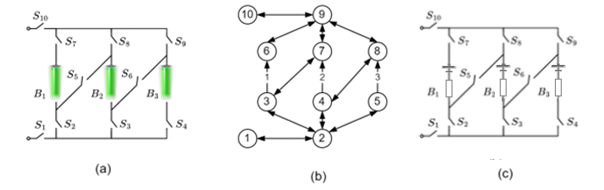
\includegraphics[width=\textwidth]{../attachments/fig2.png}
    \caption{The physical model (a), circuit model (b) and figure model(c) of the reconfigurable architecture propoesd by Visairo \cite{visairoReconfigurableBatteryPack2008}}
    \label{fig:2}
\end{figure}

\subsubsection{physical model}

The reconfigurable architecture proposed by Visairo et al.\cite{visairoReconfigurableBatteryPack2008} is shown in Figure \ref{fig:2}(a).
In this architecture, each cell is controlled by about 3 switches on average.
Excepted for two switches ($S_1$ and $S_10$ in Figure \ref{fig:2}(a)) controlling the total circuit, the vertical switches (e.g. $S_2$ and $S_7$ in Figure \ref{fig:2}(a)) allow the batteries to be directly connected to the main circuit, and the switches($S_5$ for example) in the diagonal direction can realize connecting the batteries in series.
Thus, it can dynamically change the output voltage and current as needed.
The architecture in Figure \ref{fig:2}(a) only has 3 batteries, but in practice it can add new branches containing batteries and switches to deal with large-scale batteries.

\subsection{graph model}

Figure \ref{fig:2}(b) shows the graph model based on the physical model, as shown in Figure \ref{fig:2}(a), with rules mentioned in section II.
This model captures the connection relationship between the batteries and switches, where vertex 1 and 10 represent the anode and cathode of the RBS respectively, and other vertexes represent the nodes connecting batteries and/or switches.
The directed edges marked 1, 2 and 3 refer to the corresponding batteries.
And the edges with two opposite directions represent switches.
Taking the external electrical equipment in the output circuit as a whole, a directed edge segment from $v_1$ to $v_{10}$ can be obtained. 

\subsection{circuit model}

According to the assumptions about batteries and switches in section II, an equivalent circuit model can be obtained, as shown in Figure \ref{fig:2}(c).
Based on Equation \ref{eq:A}, we can get its incidence matrix $\bm{A}$:\
{\setlength{\arraycolsep}{4pt}
\begin{equation}
\begin{array}{cc}
    &  \begin{array}{c c ccc cccccccccc} & e_o &e_{b1}  &e_{b2} & e_{b3} & e_{s1} & e_{s2} & e_{s3} & e_{s4} & e_{s5} & e_{s6} & e_{s7} & e_{s8} & e_{s9} & e_{s10} \end{array}\\
        \begin{array}{c} v_1\\v_2\\v_3\\v_4\\v_5\\v_6\\v_7\\v_8\\v_9\end{array} & \left[
    \begin{array}{c|ccc|cccccccccc}
        -1  &0 &0 &0   &1 &0 &0 &0 &0 &0 &0 &0 &0 &0\\
        0   &0 &0 &0   &-1&1 &1 &1 &0 &0 &0 &0 &0 &0\\
        0   &1 &0 &0   &0 &-1&0 &0 &1 &0 &0 &0 &0 &0\\
        0   &0 &1 &0   &0 &0 &-1&0 &0 &1 &0 &0 &0 &0\\
        0   &0 &0 &1   &0 &0 &0 &-1&0 &0 &0 &0 &0 &0\\
        0   &-1&0 &0   &0 &0 &0 &0 &0 &0 &1 &0 &0 &0\\
        0   &0 &-1&0   &0 &0 &0 &0 &-1&0 &0 &1 &0 &0\\
        0   &0 &0 &-1  &0 &0 &0 &0 &0 &-1&0 &0 &1 &0\\
        0   &0 &0 &0   &0 &0 &0 &0 &0 &0 &-1&-1&-1&1\\
    \end{array} \right]
\end{array},
\end{equation}
}
where the rows correspond to vertexes in the graph model, and the first column, second to fourth columns, and last ten columns correspond to external electrical equipment, 3 batteries, and 10 switches, respectively.
According to the above classification of the columns, the matrix $\bm{A}$ can be divided into $\bm{A}_o$, $\bm{A}_b$, and $\bm{A}_s$.


The state matrix $\bm{X}$ is determined by the switches' state, that is, the specific configuration of the RBS.
For example, when switch $S_1$, $S_2$, $S_3$, $S_4$ , $S_7$, $S_8$, $S_9$ and $S_{10}$ are closed, and switch $S_5$ and $S_6$ are open, that is , battery $B_1$, $B_2$ and $B_3$ are connected in parallel to supply power to the external circuit, the state matrix $\bm{X}$ is given by
\begin{equation}
    \bm{X} = diag(
        1,  
        \underbrace{1,1,1}_{\text{batteries}}, 
        \underbrace{1,1,1,1,0,0,1,1,1,1}_{\text{switches}}
    ).
\end{equation}


For the rest of the parameters, such as $R_o$, $r_b$ and $u_b$, this subsection still uses symbols for calculations.
Their specific value will be explained and discussed at the end of the solution.

\subsection{Module solving and discussing}

\section{Conclusion}





\bibliographystyle{ieeetr}
\bibliography{../attachments/my_ref}

\end{document}
